\chapter{Galvanic coupling for intra-body communication links} 
\section{Introduction}
Implanted sensors will enable the next generation of healthcare by in-situ testing of abnormal physiological conditions, personalized medicine and proactive drug delivery. 
The paradigm of interconnecting the implants is known as intra-body network (IBN) 
and allows implants to transmit measurements to an external processing center for real time monitoring, to receive updates on drug delivery volumes, and to directly start actions by embedded actuators. 
All these examples require energy efficient data communication between implants through body tissues.

However, the state of the art (SoA) for intra-body communication (IBC) relies on high frequency radio (RF) signals. Short-range RF communication techniques, such as Bluetooth, ANT, and Zigbee \cite{Seyedi2013} are useless for intra-body communication as they are affected by severe attenuation  within the human tissues, which are composed of 40-60$\%$ water, high power consumption, and limited battery lifetime.
Moreover, emitted RF signals propagates also around the body, creating privacy risks.  

\subsubsection{Non-RF IBC techniques}
Non-RF techniques that use the human body as a medium for data communication include ultrasound (US) technology, which consists of mechanical vibrations and works well in mediums with high water content such as the body \cite{Galluccio2012}. The main US drawbacks are severe multi-path fading and the high delay caused by slow propagation speeds. Another alternative to RF is inductive coupling (IC) \cite{Park2015}: coils wrapped around anatomy are used to generate and receive magnetic energy and the efficiency of the data transfer is directly proportional to the coupling efficiency (i.e. correct resonance frequency matching between the transmitter and the receiver), which is not always easy to achieve. Capacitive coupling (CC) \cite{Seyedi2013} uses electrical signals with a couple of electrodes at the transmitter and receiver, respectively. Only one of the electrodes at each side is attached to the body while the other electrode is floating (ground electrode needs only to be in proximity) and the signal is generated between the body channel transceiver by making a current loop through the external ground. Thus, unfortunately, the path loss has high variability based on environmental conditions.

We use an alternative cable-less architecture for IBNs using galvanic coupling (GC) technology for communications among implants.
GC utilizes low or medium frequency (1 kHz-100MHz) and weak ($< 1mW$) electrical
currents, which are modulated with data and coupled directly to the tissue \cite{Callejon2014}.
Differently from SoA RF solutions, GC IBNs does not show privacy risks since the signals do not propagate outside the body, and consumes two orders of magnitude less energy than RF method \cite{Swaminathan2016,Swaminathan2017}.

\subsubsection{Related works}
Existing GC efforts focused on signal strength changes in tissues \cite{Seyedi2013, Wegmueller2009, Callejon2014} and the characterization of human tissues \cite{Swaminathan2016, Seyedi2013, Wegmueller2010}, which are a valuable base to explor the feasibility of communication schemes that are difficult to be performed directly on the human body.

Some works have been conducted in developing GC testbeds.
For example, a test system has been designed and implemented, 
%which includes four transmitting sensors and one receiver, sending data through a frequency division multiple access (FDMA) scheme, given the costant GC attenuation over the considered frequency range, and a differential binary phase-shift-keying (DBPK) modulation, with a throughput of $4.8$ kbps  \textcolor{red}{[WEGMULLER 2009]}. 
which considers a complex programmable logic device (CPLD) containing all the digital signal processing blocks of the transmitter, and, besides the analog units, a field-programmable gate array (FPGA) at the receiver to provide the digital demodulation and interfaces \cite{Wegmueller2009}.
More recently, a base band transmission has been implemented
in a FPGA board based on impulse radio (IR) employing a pulse position modulation (PPM) \cite{Seyedi2017}.
In \cite{Tomlinson2016} design a testbed using two USRP software defined radios (SDRs), one at the transmitter and the other at the receiver side, supporting  low frequency daughterboards.
%All the aforementioned test systems are valuable works but require specific equipments and softwares, so that their corresponding experiments are not quickly replicable.
Anyhow, an effective and repeatable GC platform to carry out experiments is still a challenge. 

\subsubsection{Proposed sound card based GC testbed}
We here design and implement a GC testbed that is based on PC sound card and Matlab environment, hence easily replicable for the interested research community. The main advantages of the proposed testbed architecture are that: (i) such scheme requires limited equipment since only ordinary PCs and Matlab software are needed; (ii) allows high flexibility since all parameters, including carrier frequency, bandwidth and modulation order, may be varied directly in the TX/RX Matlab programs allowing a quick evaluation of the resulting effects; (iii) real time option for the receiver by including a Data Acquisition Toolbox (Daq Tbx) in Matlab that exploits the real time data logging feature of the toolbox \cite{Hwang2013}, so that real time transmission and evaluation of physiological data sets are possible; (iv) BER evaluation of the experimental setup. 


\section{Background on GC communication technology}
\begin{figure}
	\includegraphics[width=\textwidth]{figures/GC_testbed/GC.png}
	\caption{GC setup on skin surface with detail on multiple tissues} \label{figGCtech}
\end{figure}

An alternative ultra-low power solution that uses the human body as a communication medium is GC technology. In GC, a pair of electrodes is used to directly couple a weak electric current into the human body, so that the electrical signal is applied differentially between the two electrodes of the transmitter and secondary paths of propagation are used for potential difference detection at the electrodes of the receiver \cite{Seyedi2013}.
Recommendetion from ICNIRP \cite{Banou2018} suggests to limit the signal within the safe bound of $1$ mA, which is easily matched from GC technology, usually injecting currents in the order of $0.5$ mA \cite{Tomlinson2018}.

Fig. \ref{figGCtech} represents the conceptual illustration of GC: the transmitter is composed of a pair of electrodes with typical distance of 5 cm (on-skin case is depicted in Fig. \ref{figGCtech}, although the electrodes could be places in any tissue) to inject low intensity electrical currents as data signals. While the primary current flows through the two transmitter electrodes, weak secondary electrical currents carry the information to a distant pair of receiver electrodes using layered tissues conduction. Experiments prove that a weak secondary current can be detected at the receiver with a transmission range of 20-30 cm. GC may use any type of electrode, whose usual size is approximately 10 mm \cite{Li2017}, and consumes only 0.24 nJ per received bit compared to 106 nJ/b of Zigbee \cite{Seyedi2013}. Indeed, due to its frequency range, the GC signal is restricted to the body so that GC communication is highly energy efficient, resulting in a long lifetime for battery-powered implants. The tissue heating is low due to the limited attenuation at the frequencies used, and communication is interference-free and secure from external fields.
The operative frequency range of GC is a tradeoff among tissue attenuation, interference with other natural signals (e.g., ECG and EEG signals), and other impairments. Experiments show that the usable frequency range is 1kHz-100MHz \cite{Callejon2014}, so that other natural signals are not impaired.

\subsection{Channel Model for the human body}
\label{GCChannel}
The main approaches modeling the electrical behavior of human tissues include
wave numerical techniques, for instance, finite element analysis (FEA) and finite difference time domain method (FDTD) \cite{Wegmueller2007,Song2012}, quasi-static approximations, \cite{Pun2011,Chen2012}, and equivalent circuit analysis (ECA) models.

Field analysis with FEA and FDTD are accurate but expensive for the required time computation.
The quasi-static approximations of field distribution are less computationally complex but only model low frequency Maxwell’s equations, so that they are not valid for high frequency applications.

The ECA model gives an easy transfer function with accurate gain calculation, and is valid for a wide range of frequency.
Several ECA methods focus on single tissue layer, such as \cite{Wegmueller2010}, while a recent analytical model has been proposed that considers a three dimensional multi-layered tissue, validated through finite element simulations \cite{Swaminathan2016}.

%\textcolor{red}{An empirical GC channel model based on stored channel impulse response and analysis of the channel frequency response, noise, and capacity reveal that the channel may be modelled as additive white gaussian noise (AWGN) \cite{Tomlinson2016,Tomlinson2015}}.

\subsection{Related works on GC testbed}
%\BOOK p. 22:
Some works have been conducted to develop GC testbeds with different hardware and software features, in order to validate the aforemnetioned channel models and/or prove the GC viability as IBC technology.

%\BOOK p. 23: 
A low power single chip biomedical system is designed in [40], firstly exploiting GC paradigm, with a continuous phase frequency shift keying (CPFSK) modulation scheme.

The test system in \cite{Wegmueller2007} includes battery powered transceiver and an FPGA as interface between analog front-end and digital communication link. Two modulation schemes have been used,  frequency shift keying (FSK) and binary phase shift keying (BPSK), with a 128 and 255 kbps, respectively.

In \cite{Cho2009}, the authors build up a transceiver to communicate with both on-body and implanted sensors with a frequency range in the order of tens to hundred MHz and a data rate up to 5 Mbps. 

Base band transmissions are developed in a FPGA board based on impulse radio (IR) with a PPM, and the corresponding BER performance is evaluated  \cite{Seyedi2017}.

A GC tesbed has been proposed recently based on off-the-shelf SDR platforms with low frequency daughterboards and Matlab environment, which presents BER performance for differential BPSK (DBPSK) modulation for different level of transmitted power in case of one transmitter and one receiver implant \cite{Tomlinson2016}, and BER QPSK performance in case of two transmitters and one receiver \cite{Banou2018}.

Finally, given the heterogeneity of experimental setups and conditions, and some discrepancies observed between results in literature, some studies have been conducted to evaluate the influence of different experimental settings on GC measurements \cite{Callejon2015}.
On that purpose, different experimental setups have been considered to analyze specific key issues such as load resistance, grounding, effect of cables, and type of measurement device \cite{Callejon2015}.

Anyhow, all the developed systems require specific hardware and software and show low flexibility, resulting in GC platforms difficult to replicate for carrying out experiments.

\section{GC testbed architecture}
\begin{figure}
	\includegraphics[width=13.5cm,height=6.5cm]{figures/GC_testbed/Fig_Architecture_tot_1.jpg}
	\caption{Experimental setup of the GC testbed} \label{figGCtestbed}
\end{figure}

Since the common sound cards support signals whose frequency range is included in the GC frequency range (1KHz-100MHz), we develop and implement a GC testbed for intra-body communication links employing only ordinary PCs with sound card support and Matlab software, resulting in a simple platform to emulate a single implanted sensor transmission/reception.

The developed system may be easily reproduced and is flexible since all the parameters may easily changend in the TX/RX Matlab programs, while allowing real time transmission of physiological data sets. 
%\textcolor{red}{The Matlab-based programs for the  transmitter and receiver are available at [REFERENCE] to allow a quick implementation of the testbed for the interested researchers, and stimulate further research in the field.}
The developed testbed manages all aspects of communication, including, among the others, bit generation, preamble insertion and raised cosine filtering.


\subsection{Blocks design of the GC system architecture}
The main advantage of the proposed GC system architecture is its limited equipment requirement, consisting of two common PCs with sound card and the basic Matlab package for transmitter and receiver development, as shown in Fig. \ref{figGCtestbed} and in the block diagram in Fig. \ref{figGCaudio}. Bridging the channel and the two PCs, we ensure to use battery powered PCs without connection to the grid, in order to isolate the common ground return paths of the transmitter and the receiver, as required from GC technology \cite{Banou2018}.

Fig. \ref{figGCaudio} illustrates that only two Matlab sessions are required, one per PC, to implement the transmitter and receiver respectively, and the sound cards are used to support real signal transmission/reception in a subset frequency range of GC technology \cite{Callejon2014}. On that purpose, Fig. \ref{figGCaudio} shows that the transmitted data generated through Matlab are converted from digital to analog domain to be sent over the sound card of the transmitter. A cable is connected to the \emph{LINE OUT} jack to carry the signal outside the PC. As detailed later, the cable is attached to two electrodes that represent the GC transmitter, which send the signal over the tissue through GC communication technology. At the other side, the two receiver's electrodes bring the received signal to the other PC through the cable connected to the \emph{LINE IN} jack. The data are thus processed in the Matlab session II where the receiver program is running. 

\begin{figure}
	\includegraphics[width=\textwidth]{figures/GC_testbed/AUDIO.jpg}
	\caption{Setup of the GC audio-band testbed using two PCs} \label{figGCaudio}
\end{figure}

In the following, the blocks diagram of the proposed audio-band GC system are described, including the functional blocks of the transmitter and the receiver,  shown in Fig. \ref{figTX} and \ref{figRX}, respectively. 
%while details about the channel are given in Sec. \ref{Impl} when describing the system implementation. 

\subsection{Functional blocks of the GC transmitter}

%\textcolor{red}{specifichiamo i nomi delle variabili nella fig. 4? ma non li abbiamo tutti}\\


%The transmitter implemented in Matlab includes bit generator, BPSK modulator, preamble insertion, oversampling, raised cosine filtering, up-conversion at the carrier frequency, digital to analog conversion to send the signal over the sound card and outside the PC through a cable connected to the two electrodes of the GC transmitter. 

Before detailing each block of the transmitter shown in Fig. \ref{figTX}, we summarize in the following Table \ref{tab1} the main parameters values of the system. Note that both transmitter and receiver parameters are included for completness.

\begin{figure}
	\includegraphics[width=\textwidth]{figures/GC_testbed/TX.png}
	\caption{Block diagram of the GC transmitter} \label{figTX}
\end{figure}

\begin{table}
	\caption{Parameters setting}\label{tab1}
	\begin{tabular}{|l|c|}
		\hline
		%\textcolor{red}{ft=1;} & $\%$ symbol frequency normalized \textcolor{red}{at packet time};\\ 
		$\mathbf{Parameter}$ & $\mathbf{Value}$\\  
		\hline
		Carrier frequency $f_c$ (KHz) & $15$\\ 
		Waveform sampling frequency $f_{s_a}$ (KHz) & $48$ \\ %waveform sampling frweq whose value matches the standard  sample frequency of PC sound card
		Oversampling frequency $f_s$ in number of samples & $4$\\ %normalized at sample time Ts
		Sampling time $T_s$ (ms) & $0.16$\\
		RX oversampling frequency $f_{s_{rx}}$ in number of samples & $2$\\ %normalized at sample time Ts
		roll-off of TRX filters $R$ & $0.2$\\ 
		delay of TRX filters  $D$ in number of samples & $8$\\
		%srrc=rcosine(ft,fs,'fir/sqrt',R,delay);& $\%$ coefficients of FIR root-raised-cosine filter;\\ 
		QAM modulation order$M$ & $2$\\
		RX Wiener filter length $N_f$ in number of samples & $11$\\ 
		%length of the RX Wiener filter normalized at symbol time (with oversampling $f_{s_{rx}}=2$)
		Modulated sequence $N$ in number of symbols & $1000$\\
		Preamble length $N_{pre}$ in number of symbols & $192$\\
		\hline
	\end{tabular}
\end{table}

Fig. \ref{figTX} shows that after bit generation, a preamble is inserted and the data are modulated in BPSK. The sequence is oversampled by 4, as specified in Table \ref{tab1}, and passes through a squared-root-raised-cosine (SRRC) filter. %as transmitter pulse shape, 
The corresponding baseband samples $x(nT_s)$ are thus generated, with  $n=0,1,...,f_sN-1$ and sampling time $T_s$.

The resulting sequence is then upconverted to the carrier frequency by multiplying it by the $cos$ signal, which represents the local oscillator (LO) obtained via software-define radio in Matlab program. This yields an audio passband transmitted signal  $s_{tx}$:

\begin{equation}
s_{tx}(nT_{s_a})= x(n T_{s_a}) \cos (2 \pi f_c n T_{s_a}) 
\end{equation} 

where %$x$ is the baseband signal after oversampling and filtering, $n=0,1,...,N$, 
$T_{s_a}=1/f_{s_a}$ with $f_{s_a}=48000$ Hz, whose value is chosen according to the standard sample frequency of PC sound card, and $f_c$ is the carrier frequency. According to the parameters setting in Table \ref{tab1}, $T_{s}=8$ $T_{s_a}$ with a net data rate $R=6$ kbs, in line with several biomedical applications showing sparse and low rate traffic generated by implanted sensors \cite{Swaminathan2017,Tomlinson2018}.
%under normal physiological conditions  
Anyhow, the achievable data rate may be incresed by appropriately choosing the value of $f_s$, $f_{s_a}$, $f_c$ shown in Table \ref{tab1}. 

Fig. \ref{figTX} illustrates that the obtained audible signal $s_{tx}$ passes through the sound card's internal amplifier, which may be replaced with an external amplifier circuit using Arduino. Then, the signal is sent out to the \emph{LINE OUT} jack by using the following simple Matlab statements in Table \ref{tab2}, which play the software-generated transmitted signal:

\begin{table}
	\caption{Matlab audio playing statements}\label{tab2}
	\begin{tabular}{|l l|}
		\hline
		sObj = audioplayer($s_{tx}$,48000);&   $\%$ To create an audioplayer object for signal Stx,\\ 
		& \phantom{xx}  using sample frequency at 48000 Hz\\  
		playblocking(sObj);	& $\%$ To play from beginning till playback completes\\
		\hline
	\end{tabular}
\end{table}

Through a wire, the output signal is then connected to two electrodes, that represent the GC transmitter.

\subsection{Functional blocks of the GC receiver}

\begin{figure}
	\includegraphics[width=\textwidth]{figures/GC_testbed/RX.png}
	\caption{Block diagram of the GC receiver} \label{figRX}
\end{figure}

The main blocks of the receiver developed in Matlab are shown in Fig. \ref{figRX} and may be split in the following two macro-blocks: (i) signal recording and digital down-conversion and (ii) burst detection and symbol timing estimation.

\subsubsection{Signal recording and digital down-conversion}
A Matlab session must to be open in the PC connected with the GC receiver for running the receiver program, which includes the following Matlab statements in Table \ref{tab3} to record the received signal and store the data in the array $s_{rx}$.


\begin{table}
	\caption{Matlab recording statements}\label{tab3}
	\begin{tabular}{|l l|}
		\hline
		recObj=audiorecorder(48000,16,1); &   $\%$ To create a 48000 Hz, 16-bit, 1 channel\\ & \phantom{xx} recorder object;\\
		Tsamp=1/48000;&  $\%$ Sampling time;\\
		Trecord=$N*f_s*T_{s_a}$;&  $\%$ Recording time, where: \\ & \phantom{xx} N is the modulated sequence lenght, \\ & \phantom{xx} fs is the oversampling freq equal to 16;\\
		recordblocking(recObj,Trecord+3);&   $\%$ To record for length of time, Trecord+3,\\ &  \phantom{xx} expressed in seconds;\\
		$s_{rx}$ = getaudiodata(recObj);&   $\%$ To return the recorded audio data\\ & \phantom{xx} as a double array.\\
		\hline
	\end{tabular}
\end{table}

As shown in Fig. \ref{figRX}, after recording the signal $s_{rx}$ in digital format, which passes through the sound card amplifier, a digital down-conversion is performed by multiplying the received sampled signal by $\cos (2 \pi f_{c} n T_{s_a})$, where $f_{c}$ is the carrier frequency at the receiver. The sequence then is sent to an SRRC filter, resulting in a baseband received signal $y(nT_{s_a})$ with $n=0,1,...,f_sN-1$. 
%\textcolor{red}{(va bene mettere Ts e Tsam uguale, e variare fc e theta e awgn come disturbi?)}

The output signal is then decimated by two so that the next blocks, described below, work at two samples per symbol ($f_{s_{rx}}=2$ as specified in Table \ref{tab1}). The obtained sampled signal may be expressed as

\begin{equation}
y(nT_s)=s_{tx}(nT_s) e^{j\theta}+v(nT_s)
\end{equation}

where $n=0,1,...,f_{s_{rx}}N-1$, $s_{tx}(nT_s)$ is the envelope samples of the passband signal, $v(nT_s)$ is the sampled AWGN noise, $\theta$ is the random phase noise due to time delay. 

\subsubsection{Burst detection and symbol timing estimation}

Being the packet composed by a preamble followed by data, the burst detection is performed by estimating the start of the preamble through a correlation method.
Specifically, the transmitted preamble, known at the receiver, is cross-correlated with the receveid data so that the position of the correlation's peak gives an estimated of the preamble start position:

\begin{equation}
\hat{t}_{p}= \argmax_n \left| \sum_{k=0}^{L-1}y((n+k)T_s)p^*(kT_s)\right| 
\label{eq_delay}
\end{equation}

where $\hat{t}_{p}$ is the estimate of the sample index where the reference preamble $p$ begins, $N_{pre}$ is the preamble's length, $L=f_{s_{rx}}N_{pre}$ 
since the receiver is working at two samples per symbol (oversampling frequency $f_{s_{rx}}=2$), and $n= 0, 1,...,f_{s_{rx}}N-1$.

%cross1=xcorr(x_tot,d_pre)
%t_r1=find(cross1==max(cross1))-length(x_tot);

Hence, the received signal is shifted in time according to the estimated start of the preamble $\hat{t}_{p}$ and is equalized with a Wiener filter, that also performs symbol timing improving the delay estimate obtained with (\ref{eq_delay}). 

The coefficients $w(i)$ of the filter, with $i=1,...,N_f$, are calculated by using the shifted received preamble $y_p(nT_s)=y(nT_s+\hat{t}_{p})$ and the known transmitted one $p(nT_s)$ with $n=0,1,...,f_{s_{rx}}N_{pre}-1$.
In more details, the vector $\mathbf{w}=\left[w_1,w_2,...,w_{N_f}\right]$ of the coefficients can be computed by minimizing the mean square error (MSE) between the transmitted and estimated preamble, defined as  
%\begin{equation}
%\label{eq_MSE}
%\epsilon=E\left\{\left[x(nT_s)-\hat{x}(nT_s)\right]^2\right\}
%\end{equation}
%%with  $n=0,1,...,f_{s_{rx}}N-1$. Npre invece di N perche' uso solo preambolo, ma già detto prima. 

\begin{equation}
\label{eq_MSE}
\epsilon=E\left\{\left[p(nT_s)-\hat{p}(nT_s)\right]^2\right\}
\end{equation}

Setting the following partial derivatives of the error (\ref{eq_MSE}) equal to zero
\begin{equation}
\label{eq_deriv}
\frac{\partial \epsilon}{\partial w_i}=0, \text{  for }i=1,2,...,N_f
\end{equation}

we can solve (\ref{eq_MSE}), (\ref{eq_deriv}) for the coefficients $w_i$ by inverting an autocorrelation matrix of size $N_f\times N_f$, which leads to the following Wiener-Hopf equation
%\begin{equation}
%\label{eq_Wiener}
%\mathbf{w}=\mathbf{R}_y^{-1}\mathbf{r}_{xy}
%\end{equation}
%where $\mathbf{R}_y=\{r_y(k)\}$ is the autocorrelation matrix whose elements are $r_y(k=j-l)=E\left\{y_j(i)y_l(i)\right\} $, and $\mathbf{r}_{xy}=\{r_{xy}(k)\}$ is the cross-correlation vector whose elements are defined as $r_{xy}(k)=E\left\{x(i)y_k(i)\right\}$, and $j,l=1,2,...,N_f$.

\begin{equation}
\label{eq_Wiener}
\mathbf{w}=\mathbf{R}_{y_p}^{-1}\mathbf{r}_{py_p}
\end{equation}
where $\mathbf{R}_{y_p}=\{r_{y_p}(k)\}$ is the autocorrelation matrix of the received preamble $y_p$, whose elements are $r_{y_p}(k)=E\left\{y_{p}(i-k)y_{p}(i)\right\} $, and $\mathbf{r}_{py_p}=\{r_{py_p}(k)\}$ is the cross-correlation vector between the transmitter preamble $p$ and the received one $y_p$, whose elements are defined as $r_{py_p}(k)=E\left\{p(i-k)y_{p_k}(i)\right\}$, and $i,k=1,2,...,f_{s_{rx}}N_f$.

After calculating the Wiener coefficients using only the preamble, the filter is applied to all the sequence, so that its output is the estimated transmitted sequence $\hat{x}(nT_s)$, expressed as
\begin{equation}
\label{eq_outW}
\hat{x}(nT_s)=\sum_{l=0}^{N_f-1}w(lT_s)y((n-l)T_s+\hat{t}_{p})
\end{equation}

%Note that, since we are employing the Wiener filter in place of a matched Nyquist filter, we have $N_f=2q+1$ where $q$ is the number of the finite impulse response (FIR) Wiener coefficients, so that $\mathbf{w}$ may be expressed as $\left[w_{-q},...,w_{0},...,w_{q}\right]$ and $r_{xy}(k)=\sum_{l=-q}^{q}w(l)r_y(k-l)$, with $k=-q,...,q$.










%\textcolor{red}{filtro Wiener (sostitusce srrc) è adattativo (invece srrc è adattato) e fa insieme 3 cose: equalizza (se i coeff dei filtri fanno qualcosa in freq), recupero fase, e timing di clock (diverso da timimg di pacchetto che stimiamo con synchro con max correlaz); uso inviato filtrato due volte (dd) e ricevuto con awgn che viene filtrato due volte (sn2)}

After a downsampling operation at one sample per symbol, the BPSK symbol sequence is demapped to a bit sequence and the preamble is removed, thus completing the receiver operations. The obtained bit sequence may be hence compared to the transmitted one for BER calculation.
 
\subsection{Implementation of the GC system}
\label{Impl}
%\textcolor{red}{AWGN se senza filo ma solo programmi con dati inviati salvati?}
Before evaluating the performance of the overall system with a real tissue-based GC channel, we first test only the transmitter and the receiver, for which the configuration in Fig. \ref{FigWIRE} is considered. Then, 
%a simulated channel is included in such setting, and finally 
an experimental setup is evaluated with real tissue for GC transmissions as in Fig. \ref{figGCaudio}. 

Fig. \ref{FigWIRE} derives from Fig. \ref{figGCaudio} by substituting the steak with a simple wire connecting the \emph{LINE OUT} sound card's jack of the PC running the Matlab transmitter program with the \emph{LINE IN} jack of the other PC running the receiver program.
\begin{figure}
	\includegraphics[width=\textwidth]{figures/GC_testbed/AUDIO_WIRE.jpg}
	\caption{Audio-band testbed using two PCs and a wire} \label{FigWIRE}
\end{figure}

%\subsubsection{GC system with simulated channel}
%\textcolor{red}{As specified in Sec. \ref{GCChannel}, the behavior of the GC channel may be simulated through an additive white gaussian noise (AWGN) channel \cite{Tomlinson2016,Tomlinson2015}.} 
%The proposed sound-card based testbed will be used also to validate such empirical results.
%Specifically, considering the setting in Fig. \ref{FigWIRE}, the channel is modeled with a delay on the received signal and an AWGN, whose Matlab commands are included in the receiver program after the recording statements. 
For the final setting, shown in
Fig.  \ref{figGCtestbed} and \ref{figGCaudio},
%We simulate the GC channel in the setting of Fig. \ref{FigWIRE} by introducing a delay on the received signal and applying an AWGN. The corresponding Matlab commands are included in the receiver program after the recording statements specified in Table \ref{tab3}. Sec. \ref{Exp} shows the performance of the proposed architecture in such setting as first evaluation test.
%\subsubsection{GC system with experimental channel}
%The proposed architecture 
the wire connecting \emph{LINE IN} and \emph{LINE OUT} jacks of the two PCs is cutted and each of its two parts are attached to the electrodes of the GC transmitter and receiver, respectively. Since the wire is composed by three electric clables, two of them are connected to the electrods on each side, while the third one remains floating. Under this configuration, the two transmitter and receiver Matlab session runs in parallel to perform the experimental evaluation detailed in the following section.




\section{Experimental Setup and Performance Evaluation}
\label{Exp}
%\textcolor{red}{Ptx max 12 mW per cui se metto volume al 70$\%$ ho 8.4 mW}

After testing the architecture in the configuration shown in Fig. \ref{FigWIRE}, which have confirmed the feasibility of the proposed transmitter and receiver architecture, we have conducted experiments in the final real scenario shown in Fig. \ref{figGCtestbed} and Fig. \ref{figGCaudio}. 
The parameters setting is detailed in Table \ref{tab1}, and the average BER is calculated over $100$ iterations. 

Note that we use really small size electrodes (in the order of $0.5$ mm) while the SoA is employing $1$ cm electrodes \cite{Li2017}. Although such choice would reduce the achievable distance between GC transmitter and receiver, in this way we test a real configuration scenario for future miniaturized implantable devices. 
The inter-distance between the electrodes at both the transmitter and receiver is set equal to $1$ cm, while the distance between the transmitter and receiver is varied during the experiments, together with the transmit power.

\begin{figure}
	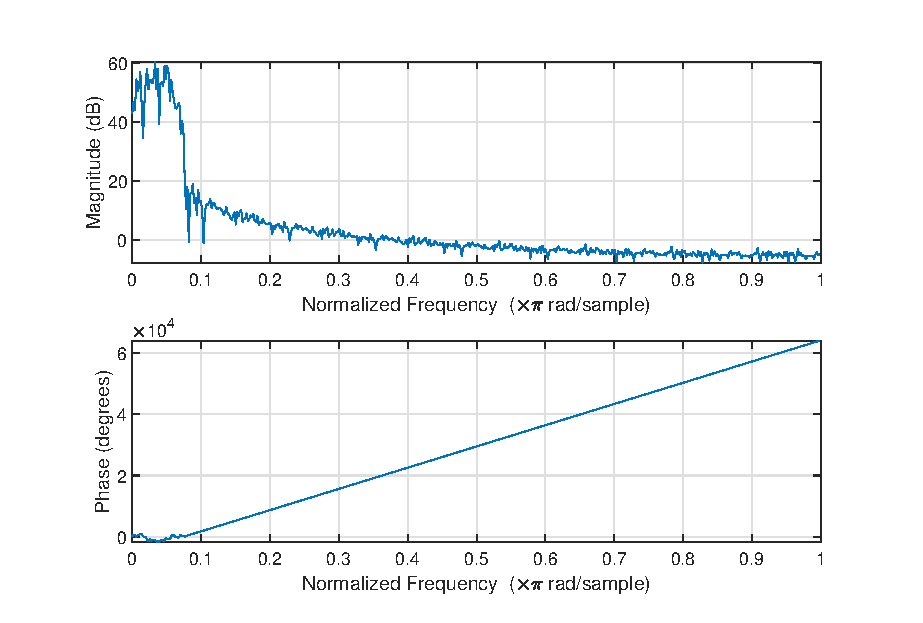
\includegraphics[width=\textwidth]{figures/GC_testbed/TX_freq.eps}
	\caption{Transmitted signal in frequency domain} \label{FigTXfreq}
\end{figure}

\begin{figure}
	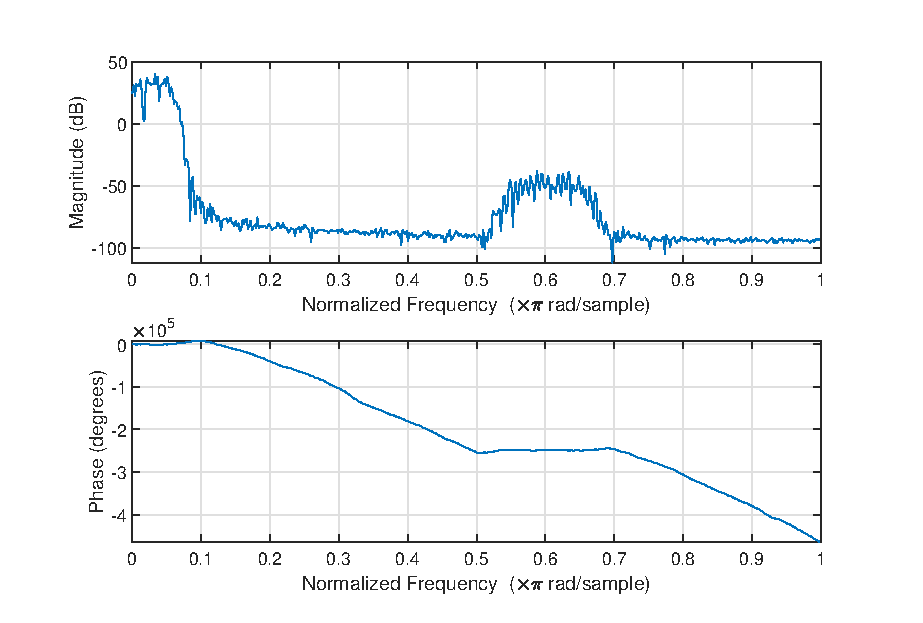
\includegraphics[width=\textwidth]{figures/GC_testbed/RX_freq}
	\caption{Received signal after RX filter in frequency domain} \label{FigRXfreq}
\end{figure}

Fig. \ref{FigTXfreq} and Fig. \ref{FigRXfreq} show the transmitted and received signal in the frequency domain, respectively, for $3$ cm distance between GC transmitter and receiver. Fig. \ref{FigTXfreq} refers to the transmitted signal before being modulated on the carrier frequency, as well as Fig. \ref{FigRXfreq} illustrates the received signal after demodulation and filtering. The comparison between the two figures confirms that the received signal exibiths the same shape of the transmitted one, since the side lobe of the receiver signal is maintained low by the filter being its amplitude around $90$ dB less than the main one. 
%The difference in the phase between the two transmitted and received signals is due to the time delay, which is correctly detected and compensated only in the block after the RX filter, while Fig. \ref{FigRXfreq} shows the signal before such compensation (see the receiver blocks in Fig. \ref{figRX}).     

\begin{figure}
	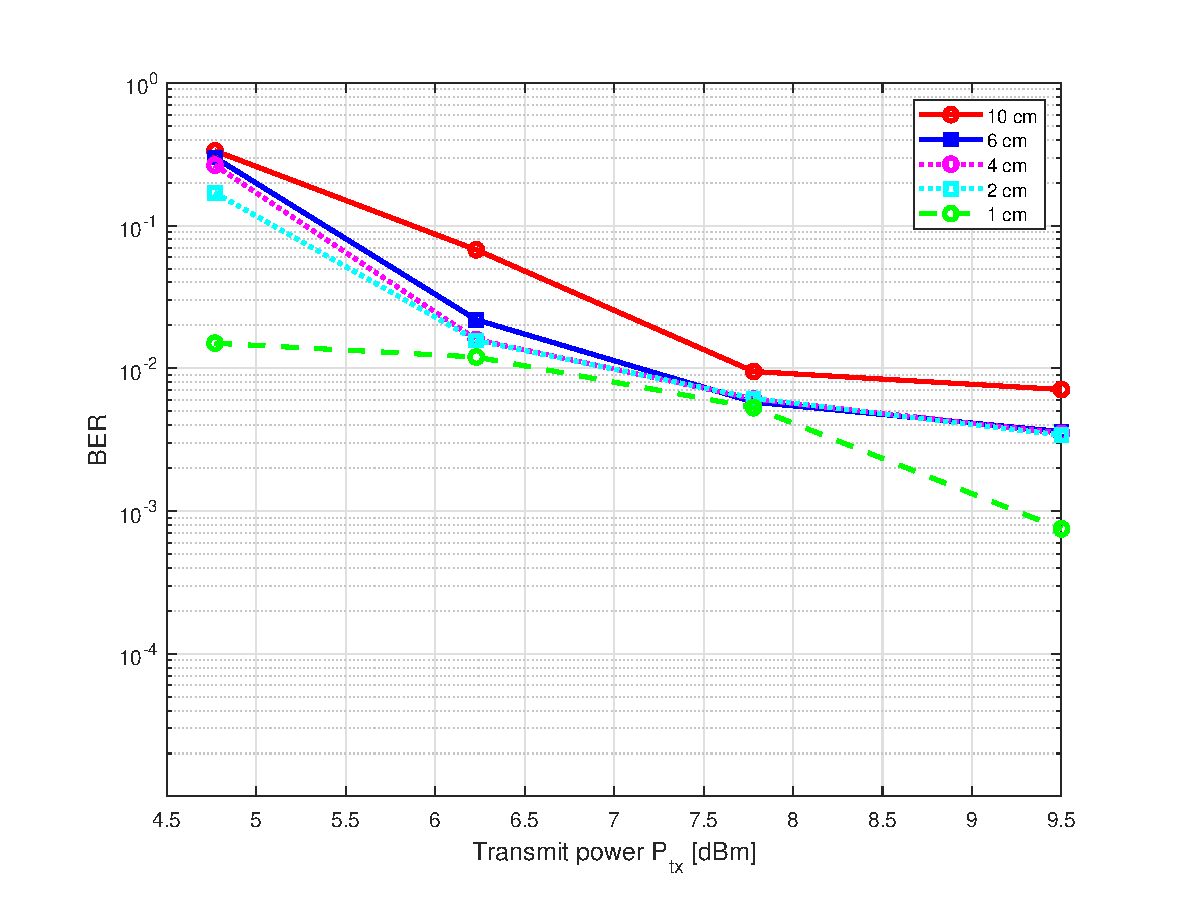
\includegraphics[width=0.85\textwidth]{figures/GC_testbed/BER_TXpower}
	\caption{BER vs transmit power for different distances between GC transmitter and receiver} \label{FigBER}
\end{figure}

Fig. \ref{FigBER} shows BER performance by varying the transmit power for different distance values between transmitter and receiver. As expected, BER performance decreases when increasing the distance, although the performance for $2$, $4$, $6$ cm result to be quite similar. We are able to achieve a BER in the order of $10^{-4}$ with $9.5$ dBm transmit power for $1$ cm distance, reaching $7 \cdot 10^{-3}$ for $10$ cm, a valuable result considering the small electrode size of $0.5$ mm and the simple receiver that is not employing any correction code. More robust receiver may be envioned based on ultra wideband (UWB) to improve the performance while mantaining simple and energy efficient receiver \cite{Alesii2015}, as required by biomedical implantable devices.    


\section{Conclusions}

We have proposed a sound card based GC testbed as a quick repeatable platform to carry out experiments. The detailed description of the implemented test system may support the interested researchers in replicating the testbed and thus stimulate further research in the GC field.
Experimental tests on real chicken tissue as GC communication channel have been conducted to prove the feasibility of the proposed architecture.
We achieve a BER in the order of $10^{-3}$ with  $9.5$ dBm transmit power for distances in the range $2-10$ cm, employing an simple receiver and electrodes with really small size ($0.5$ cm), while the SoA is usually employing $1$ cm electrodes.
Ongoing works include exstensive simulation to evaulate the effect of the carrier frequency, bandwidth, audio sampling frequency, electrodes size, as well as inter-electrodes distance at both the transmitter and receiver. Moreover, we are implementing an extension of the proposed testbed with Arduino platform in order to modulate the signals on a frequency range larger than the audio signals. Future research directions will exploit compressed sensing (CS) and UWB techniques to save time and energy \cite{Banou2018,Alesii2015}, a strict requirements in intra-body networks for medical applications.